\documentclass[8pt,aspectratio=169,fleqn]{beamer}

\usepackage[utf8]{inputenc}
\usepackage[T1]{fontenc}
\usepackage{lipsum}
\usepackage{bm}
\usepackage{booktabs}
\usepackage{appendixnumberbeamer}

\usetheme{spc}

\title{Existence of Electromagnetic-Hydrodynamic Waves}
\date[]{28 June 2019}
\institute{École Polytechnique Fédérale de Lausanne -- Swiss Plasma Center}
\author[H. Alfvén]{Hannes Alfvén\\{\small hannes.alfven@epfl.ch}}

\begin{document}
\begin{frame}[plain]
\titlepage
\end{frame}

\begin{frame}
  \frametitle{A title for this frame}
  \framesubtitle{And a subtitle}

  Lorem ipsum dolor sit amet, consectetur adipiscing elit. Nunc
  semper dui vitae lacus rutrum, et ullamcorper massa pharetra.

  \begin{itemize}
  \item Aliquam malesuada ac odio vitae vehicula. Quisque sodales quam ac accumsan mattis.
  \item Morbi in nulla quam. Fusce nec luctus risus, quis accumsan tortor.
  \item Curabitur tortor justo, fermentum sit amet finibus nec, pulvinar nec arcu.
  \item Proin quis lorem bibendum nunc suscipit molestie. Integer tortor sem, porta ut tincidunt id,
    faucibus pellentesque magna.
  \end{itemize}
\end{frame}

{
  \usebackgroundtemplate{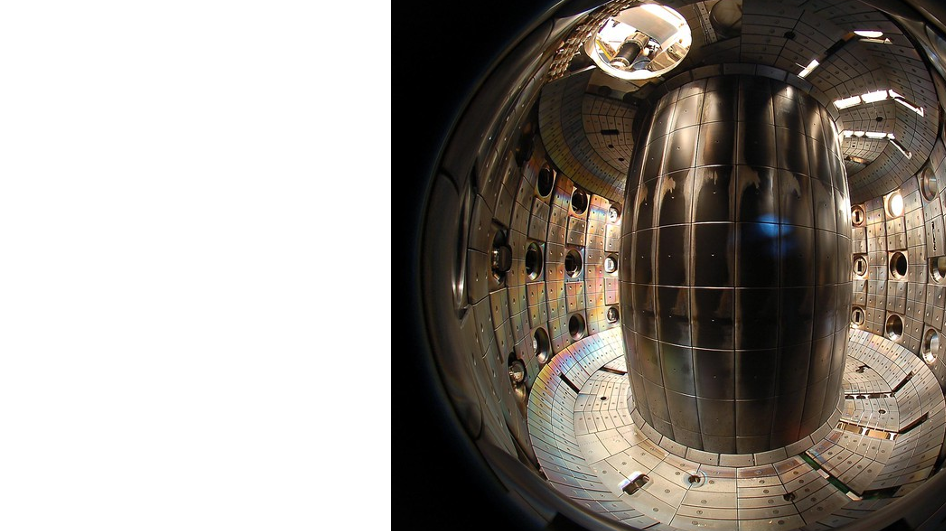
\includegraphics[width=\paperwidth]{figures/TCV_bg}}
  \begin{frame}
    % \frametitle{An improved hybrid electron model}
    \begin{tikzpicture}
      % Define bounding box
      \useasboundingbox (0,0) rectangle(\the\paperwidth,\the\paperheight);
      % Define title page
      % Put main background image
      \fill[color=greyEPFL, anchor=south west] (2,3.25) rectangle (7.50,4.75);
      \fill[color=redEPFL, anchor=south west] (0,1.55) rectangle (2.00,3.25);
      \fill[color=greyEPFL, anchor=south west] (2,0.00) rectangle (4.25,1.55);
      \node[anchor=west, white,font=\large, align=left] at (2,4.0){\textbf{A transition slide}};
    \end{tikzpicture}
  \end{frame}
}

\begin{frame}
  \frametitle{A frame without subtitle}
  \framesubtitle{}
\end{frame}

{
  \usebackgroundtemplate{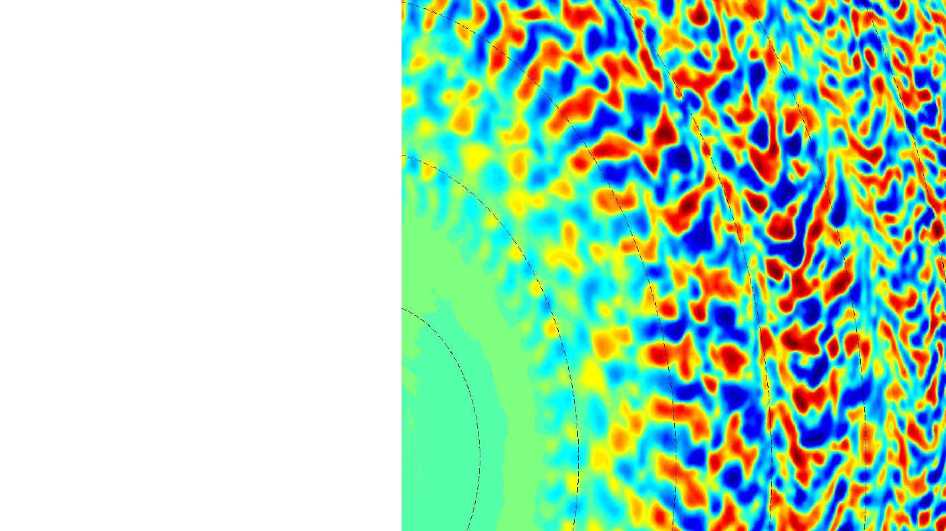
\includegraphics[width=\paperwidth]{figures/turb_bg2}}
  \begin{frame}
    % \frametitle{An improved hybrid electron model}
    \begin{tikzpicture}
      % Define bounding box
      \useasboundingbox (0,0) rectangle(\the\paperwidth,\the\paperheight);
      % Define title page
      % Put main background image
      \fill[color=greyEPFL, anchor=south west] (2,3.25) rectangle (7.50,4.75);
      \fill[color=redEPFL, anchor=south west] (0,1.55) rectangle (2.00,3.25);
      \fill[color=greyEPFL, anchor=south west] (2,0.00) rectangle (4.25,1.55);
      \node[anchor=west, white,font=\large, align=left] at (2,4.0){\textbf{An other transition slide}};
    \end{tikzpicture}
  \end{frame}
}

\begin{frame}

\end{frame}
\end{document}
